\subsubsection{Rodzaje przedmiotów do interakcji}
Ze względu na charakterystykę gatunku gry, główną częścią interaktywnych obiektów stanowią bronie.
Zaimplementowane w grze zostało 5 broni (2 z nich występują w różnych wariantach kolorystycznych):
\begin{itemize}
    \item Pistolet (warianty czarny, biały, brązowy)
    \item Rewolwer
    \item Strzelba
    \item Karabin (warianty jak pistolet)
    \item Karabin Sniperski
\end{itemize}

Wprowadzone zostały również obiekty powiązane z mechanikami w grze:
\begin{itemize}
    \item Apteczka - w celu uzupełniania punktów zdrowia - występują obecnie dwa warianty - bazujące na takim samym meshu, lecz używające innej tekstury
    \begin{enumerate}
        \item Czarna - odnawia 15 \% maksymalnych punktów zdrowia
        \item Czerwona - odnawia 35 \% maksymalnych punktów zdrowia
    \end{enumerate}
    \item Skrzynka z amunicją - po wejściu w interakcje sprawdza ilość amunicji gracza, jeżeli jest ona różna od maksymalnej (przez maksymalną rozumie się trzykrotność pojemności magazynka) dla dowolnej z broni noszonej przez gracza - pozwala na uzupełnienie amunicji do ilości maksymalnej
    \item Pancerz - po wejściu w interakcje sprawdza obecną wartość pancerza gracza - jeżeli jest różna od 100\%, uzupełnia ją do maximum
    \item Gaz - interakcja odbywa się nie jak w wszystkich powyższych - przez odpowiedni klawisz - lecz przez wejście gracza w zakres collidera. \\
    Wejście w zakres collidera odpala funkcje zadającą bohaterowi obrażenia w czasie.
    \item Szkło - została zaimplementowana możliwość rozbijania obiektów.//
    Żeby tego dokonać, za pomocą kodu obiekt szkła sprawdza za pomocą collidera kolizje z pociskami wystrzelonymi przez gracza/bota.\\
    W momencie wykrycia takowej kolizji następuje eksplozja niszcząca szkło oraz podmiana prefabu na odłamki szkła.\\
    Otwiera to szerokie spektrum możliwości w kontekście tworzenia poziomu - bowiem zniszczenie takowego szkła posiada również towarzyszący temu dźwięk - co może informować gracza o obecności przeciwników.
    Dodatkowo, otwiera to możliwość strzelania przez przestrzenie które nie są blokowane szkłem po zniszczeniu go.
    \item Skrzynie z granatami - zasada działania jest podobna do skrzyni z amunicją ( tutaj maksimum dla danego typu granatu wynosi 3) - jednak sprawdza ona wszystkie z 3 możliwych typów granatów
    \begin{enumerate}
        \item Wybuchowy - warto wspomnieć że on również jest w stanie wchodzić w interakcje z szkłem tj. niszczyć
        \item Dymny - po rzuceniu triggeruje się Particle Effect, tworzący dym na małym obszarze
        \item Hukowo-błyskowy - po rzuceniu, wybucha, w momencie kiedy gracz patrzy w kierunku granatu w momencie, na ekranie zostaje wyświetlony biały canvas zasłaniający cały ekran, który wraz z czasem zanika (poprzez obniżanie jego wartości alpha), dodatkowo wybuchowi towarzyszy głośny dźwięk
    \end{enumerate}
    \item Skrzynie\\\ trumny - wejście w interakcje triggeruje animacje otwarcia skrzyni (lub trumny), wewnątrz której można znaleźć broń (nie każda skrzynia zawiera broń, obiekty broni są dodawane ręcznie do owych skrzynek)
    \end{itemize}
Oprócz wyżej wymienionych elementów związanych z mechanikami, gracz może wejść również w interakcje z:
    \begin{itemize}
        \item drzwiami przesuwnymi - otwierają się w momencie wejścia w kolizje z colliderem gracza
        \item drabiną - podejście pozwala na wspinanie się gracza w celu uzyskania dostępu do wybranych lokacji
        \item bramą - wejście w interakcje otwiera ją, umożliwiając graczowi wejście na cmentarz
    \end{itemize}
\subsubsection{Sposób implementacji}
Wszystkie z powyższych interaktywnych obiektów zostały przygotowane jako prefaby, z podpiętymi wszystkimi niezbędnymi komponentami oraz skryptami \\
Następnie owe prefaby zostały wkomponowane w poziom, z uwzględnieniem balansu poprzez rozmieszczenie słabszych broni w łatwiej dostępnych lub bardziej oczywistych lokacjach, natomiast potężniejsze wyposażenie zostało ukryte w skrzyniach w cięższych do osiągnięcia lokacjach (przez trudność dostania się do lokacji rozumiane jest albo wyzwanie pod kątem zręcznościowym - wymaga skoków i odpowiedniego poruszania, lub spora ilość przeciwników w danej lokacji)
Wyjątkiem od wyżej wymienionej zasady jest gaz - który został użyty jako immersyjny sposób do ograniczenia wielkości poziomu.

\begin{figure}[h]
        \centering
        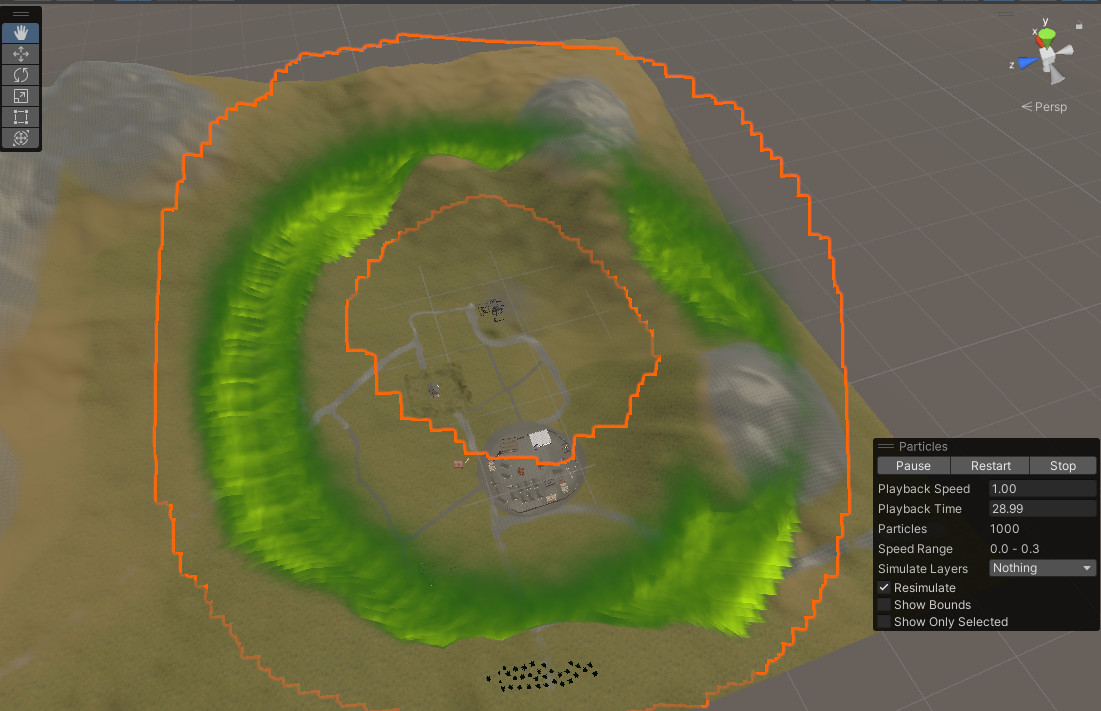
\includegraphics[width=1\linewidth]{Images/gas.png}
        \caption{Zastosowanie gazu jako naturalnego ograniczenia wielkości poziomu}
\end{figure}

